\chapter{Quantifying sensitivities of satellite-simulated cloud
retrievals to unresolved clouds and precipitation}\label{sec:subgrid1}

The simulator framework is essentially a means for accounting for
uncertainties, biases, and limitations in satellite retrievals of cloud
properties in order to make more consistent comparisons with modeled
cloud properties. However, because the descriptions of clouds in GCMs
are themselves limited and insufficient for directly simulating the
satellite retrievals, the process of simulating satellite retrieval
products relies on additional assumptions about the model clouds beyond
the descriptions provided by the models themselves. This introduces
another layer of complexity and another possible source for errors or
ambiguities.

At the heart of this problem is the fact that while cloud properties in
the physical atmosphere vary at all spatial scales down to (and below)
those measured by satellite sensors, the current resolution of most
global climate models is limited by computational expense and model
infrastructure to hundreds of kilometers. For example, climate model
simulations produced for the latest round of the Climate Model
Intercomparison Project (CMIP5; {[}citations{]}) and referenced in the
Intergovernmental Panel on Climate Change (IPCC) AR5 used grids with
typical resolutions of 1 to 2 degrees \citep{flato_et_al_2013}, which
translates to about 100-200 km at the equator. Because of these
coarse-scale grids, current large-scale models cannot explicitly resolve
individual cloud elements at the scales observed by satellites (1-2 km
for the MISR and CloudSat retrievals used predominantly in this study),
but rather must rely on (often empirically-based) statistical
parameterizations about the nature of clouds at these larger scales that
summarize the aggregated properties of the smaller scales
\citep{randall_et_al_2003}.

As stated by \citet{pincus_et_al_2012} and mentioned in
Section~\ref{sec:introductionChapter}, the relatively coarse resolution
of GCMs is problematic because the gridbox-mean description of clouds
implies a distribution of possible simulated retrievals within each
gridbox. The gridbox mean description of clouds does not in itself
specify how the clouds should be distributed horizontally and vertically
within model gridboxes, and thus characterization of the unresolved
structure depends on additional assumptions about how clouds in
overlapping layers are aligned vertically and how cloud properties vary
within model gridboxes.

The importance of unresolved cloud properties is not unique to the
problem of simulating satellite retrievals, but is more generally
important to the problem of calculating radiative fluxes and heating
rates within models. This is due to the fact that radiative fluxes are
non-local. That is, the radiative flux resulting from a combination of
two layers depends on the degree to which those two layers overlap
vertically. Many early radiative transfer parameterizations in
large-scale models accounted for the overlapping nature of clouds from
partly cloudy layers by appropriately weighting clear and cloudy-sky
flux calculations to satisfy a specific overlap assumption. These
overlap assumptions were necessarily simply defined, and have included
random overlap, in which clouds in different vertical layers are assumed
to be completely uncorrelated, maximum overlap, in which clouds in
different layers are assumed to be perfectly correlated (or ``lined
up''), and the popular maximum-random overlap, in which clouds in
adjacent cloudy (or continuous) layers are maximimally overlapped and
clouds in layers separated by at least one clear layer are randomly
overlapped \citep{geleyn_and_hollingsworth_1979, tian_and_curry_1989}.
The maximum-random overlap in particular has been used in a number of
GCMs
\citep[e.g.;][]{collins_et_al_2004, neale_et_al_2010a, neale_et_al_2010b}.
That different overlap assumptions can significantly affect simulated
radiative quantities is well established
\citep[e.g.,][]{morcrette_and_fouquart_1986, stubenrauch_et_al_1997, barker_et_al_1999},
and these overly simple assumptions have been shown insufficient in
capturing the complexity of cloud overlap seen in observations
\citep{hogan_and_illingworth_2000, mace_and_benson-troth_2002, barker_2008}
and in high-resolution model simulations {[}citations{]}. Sensitivity
tests using high resolution model simulations have shown that these
unrealistic overlap assumptions can lead to instantaneous errors in
calculated fluxes in excess of \(50 \textrm{W/m}^2\)
\citep{barker_et_al_1999, wu_and_liang_2005}, suggesting that a more
realistic treatment of cloud overlap should be sought for inclusion in
GCMs. Subgrid-scale horizontal variability in cloud condensate is often
completely neglected (or poorly represented by simple scaling of optical
depths, e.g. {[}citations{]}) in GCMs, despite the fact that clouds can
exhibit large horizontal variability on scales much smaller than GCM
gridboxes \citep[e.g.;][]{stephens_and_platt_1987}. This is problematic
because radiative fluxes and heating rates calculated from model
radiative transfer parameterizations are sensitive to subgrid-scale
variations in cloud condensate
\citep[e.g.,][]{barker_et_al_1999, wu_and_liang_2005, oreopoulos_et_al_2012}.
\citet{barker_et_al_1999} demonstrate instantaneous flux errors due to
unresolved horizontal cloud variability in excess of 100
\(\textrm{W/m}^2\), and \citet{oreopoulos_et_al_2012} demonstrate global
cloud radiative effect errors on the order of 5 \(\textrm{W/m}^2\), with
much larger regional errors. The sensitivity to both cloud overlap and
condensate horizontal variability emphasizes the need to provide
descriptions of clouds in large-scale model radiative calculations that
include both horizontal variability in cloud properties and more
realistic cloud overlap.

An alternative to the approach of weighting clear and cloudy sky fluxes
is to generate stochastic samples of binary clear or cloudy
``subcolumn'' profiles, in which each subcolumn element has either unit
or zero cloud fraction, and in the limit if many such samples the
gridbox-mean partial cloudiness profile is reproduced and the subcolumn
profiles are consistent with an assumed overlap. This approach,
described by \citet{klein_and_jakob_1999} to generate stochastic
subcolumns for use with the ISCCP simulator, provides psuedo-resolved
cloud fields sufficient for not only simulating satellite retrievals,
but also for performing radiative transfer calculations using the
independent column approximation \citep[ICA;][]{cahalan_et_al_1994}.
\citet{pincus_et_al_2003} made this approach for calculating fluxes and
heating rates much more tractable for use in large-scale models by
introducing the Monte Carlo Independent Column Approximation (McICA), in
which both cloud state (subcolumns) and spectral interval are
stochastically sampled simultaneously, drastically reducing the
computational burden associated with integrating calculations over a
large number of spectral intervals for each column. This allows for fast
ICA-like radiative transfer calculations (at the expense of artificially
increased random noise) and more flexible representations of
subgrid-scale cloud structure, and has since been incorporated into the
widely used RRTMG radiation package and used in a number of
state-of-the-art models
\citep{iacono_et_al_2008, von_salzen_et_al_2012, neale_et_al_2010a, neale_et_al_2010b, donner_et_al_2011, hogan_et_al_2014}.

McICA separates the treatment of cloud structure and variability from
radiative transfer parameterization, leaving the task of describing
complex cloud structure and variability up to subcolumn sampling
schemes. In principle, arbitrarily complex cloud geometries and
condensate distributions can be generated by incorporating more
sophisticated subcolumn schemes. However, the subcolumn schemes
currently used in most GCMs make many of the same simplifications used
by earlier models, including maximum-random overlap and homogeneous
cloud properties \citep[e.g.;][]{neale_et_al_2010a, neale_et_al_2010b}.
Improved subcolumn schemes are needed to take full advantage of the
flexibility offered by McICA.

As discussed in Section~\ref{sec:introductionChapter}, the first step in
simulating satellite retrievals from GCM output is to downscale the
gridbox-mean quanitities to scales approximating those at which the
actual satellite retrievals are performed. In COSP, this is done by
generating stochastic subcolumns following \citet{klein_and_jakob_1999},
analogous to how subcolumns are generated for McICA, following the
simple overlap assumptions described above with horizontally homogeneous
cloud condensate. To the extent that the simulated satellite retrievals
are sensitive to these assumptions, failing to accurately characterize
the subgrid cloud structure and condensate variability potentially
introduces ambiguities into satellite-model comparisons. The sensitivity
of the satellite-simulated cloud properties to assumptions about
unresolved cloud and precipitation are quantified here, and a framework
for reducing errors due to these assumptions is presented in
Section~\ref{sec:subgrid2}.

\section{Generating stochastic subcolumns of cloud and
precipitation}\label{generating-stochastic-subcolumns-of-cloud-and-precipitation}

\{\#sec:subgrid1Scops\}

As described by \citet{bodas-salcedo_et_al_2011}, the individual
instrument simulators in COSP require profiles or columns of cloud and
precipitation in which cloud and precipitation fraction is either zero
or one at each level (i.e., profiles of binary cloud and precipitation
occurrence). Because large-scale models (GCMs and numerical weather
prediction models or NWPs) do not resolve clouds, this requires
inferring these profiles of resolved cloud and precipitation occurrence
using an ensemble of subcolumns for each model gridbox. As stated by
\citet{bodas-salcedo_et_al_2011}, these subcolumns can be provided by
the model if available, as may be the case if the model uses such
subcolumns elsewhere in the code, such as in an implementation of McICA
for calculating radiative fluxes as described above. But, if such
subcolumns are not available (as may be the case even if McICA is used
in the radiative transfer part of the model, due to model infrastructure
challenges), COSP contains code for generating subcolumns itself using
the model large-scale description of clouds.

Generating stochastic subcolumns of cloud and precipitation properties
is itself a multi-step process. First, stochastic subcolumns of binary
cloud occurrence are generating using the Subcolumn Cloud Overlap
Profile Sampler (SCOPS), described conceptually by
\citet{klein_and_jakob_1999} and \citet{webb_et_al_2001}. SCOPS can
generate subcolumns obeying random, maximum, or maximum-random overlap,
and can separately treat convective and stratiform cloud if such a
distinction is made in the model. If the model distinguishes between
convective and stratiform cloud, convective cloud is maximally
overlapped and the remaining stratiform cloud may follow a separate
overlap assumption (one of random, maximum, or maximum-random) in SCOPS,
as described by \citet{webb_et_al_2001}. SCOPS takes as input the
gridbox-mean total cloud fraction profile \(\overline{c}_k\) (the
fraction of the gridbox at each level \(k\) containing either stratiform
or convective cloud) and the gridbox-mean convective cloud fraction
profile \(\overline{c}^\textrm{conv}_k\), and outputs an ensemble of
\(n_\textrm{col}\) binary subcolumn cloud occurrence profiles
\(c_{i, k}\), where for each subcolumn \(i\) and at each level \(k\),
\[\begin{gathered} c_{i, k} = \begin{cases} 0 &
~\text{if subcolumn is clear} \\ 1 & ~\text{if subcolumn is stratiform cloud} \\
2 & ~\text{if subcolumn is convective cloud} \end{cases}\end{gathered}\]

Following the generation of subcolumn cloud occurrence profiles,
subcolumn binary precipitation occurrence profiles are generated
following the algorithm described by \citet{zhang_et_al_2010} and
implemented in the PREC\_SCOPS routine within COSP. PREC\_SCOPS takes as
input the subcolumn cloud occurrence (stratiform and convective) as
determined by SCOPS and either the gridbox-mean precipitation condensate
amount (mixing ratio) or the gridbox-mean precipitation fluxes. Again,
PREC\_SCOPS handles large-scale (resulting from stratiform cloud) and
convective precipitation separately if the model distinquishes between
the two. The following paraphrases the description of the algorithm in
\citet{zhang_et_al_2010}. The algorithm steps down through model levels
from the top of the atmosphere to the surface. Large-scale precipitation
is first assigned to to all those subcolumns that have non-zero
large-scale precipitation (condensate or flux) in the current level and
either stratiform cloud (as determined by SCOPS) in the current level,
or non-zero gridbox-mean large-scale precipitation (condensate or flux)
in the level above. If large-scale precipitation is non-zero but is not
assigned by these two criteria, the algorithm assigns precipitation to
all subcolumns with stratiform cloud in the level below. If large-scale
precipitation is non-zero but is not assigned by these three criteria,
it is assigned to all subcolumns with stratiform cloud anywhere in the
vertical column. If large-scale precipitation is non-zero but has not
been assigned by any of these criteria, it is assigned to subcolumn in
the current level. This procedure is repeated for convective
precipitation (replacing stratiform in the above rules with convective
cloud), but in the case that precipition is not assigned by the first
four criteria it is assumed to only cover 5\% of the subcolumns for
convective precipitation, as opposed to filling all subcolumns in the
case of large-scale precipitation.

Once subcolumn profiles of binary cloud and precipitation occurrence
have been generated, condensate amounts (mixing ratios) are assigned to
the cloudy and precipitating elements. The current implementation in
COSP assumes a constant in-cloud (and in-precip) condensate mixing ratio
at each level within each gridbox, so that each subcolumn at a given
level within a gridbox is assigned the same in-cloud (or in-precip)
condensate mixing ratio. The in-cloud condensate mixing ratio for a
specific hydrometeor type (i.e., stratiform cloud liquid, stratiform
cloud ice, convective cloud liquid, or convective cloud ice)
\(\tilde{q}_k\) at level \(k\) is calculated from the gridbox mean
mixing ratio \(\overline{q}_k\) by dividing the gridbox-mean condensate
mixing ratio by the fraction of subcolumns containing cloud of that type
(stratiform or convective) at that level,
\(a_k = \sum_{i = 1}^{n_\textrm{col}} c^\prime_{i, k} / n_\textrm{col}\),
where \(c^{\prime}_{i, k}\) is the subcolumn binary cloud occurrence for
the particular hydrometeor type (\(c^\prime = 1\) where either \(c = 1\)
for stratiform or \(c = 2\) for convective, and \(c^\prime = 0\)
otherwise) and \(n_\textrm{col}\) is the number of subcolumns, so that
\[\begin{gathered}
\tilde{q}_k = \overline{q}_k / a_k\end{gathered}\] This is then repeated
for precipitation, using the precipitation subcolumn profiles generated
by PREC\_SCOPS.

The precipitation treatment described above attempts to associate
precipitation with cloud, but fails to account for any estimate of
precipitation fraction (the fraction of the gridbox that contains
precipitation at any level) that may be diagnosed by the model. As will
be shown in the following sections, this can lead to a gross
over-estimation of the number of precipitating subcolumns using the
\citet{zhang_et_al_2010} algorithm, and consequently a gross
over-estimation of the occurrence of large values of simulated radar
reflectivity factor. An adjustment to the subcolumn precipitation
occurrence is added here, following the work of
\citet{dimichele_et_al_2012}, in which subcolumn precipitation is either
added or removed at each level until the fraction of subcolumns with
precipitation at a given level matches the input precipitation fraction.
Precipitation is added preferentially to columns with more (vertically
integrated) cloudy levels, and removed preferentially to columns with
less cloudy levels. This is similar to the ``PEVAP'' adjustment
described by \citet{dimichele_et_al_2012}, and the improvement to
simulated radar reflectivity in response to this adjustment will be
evaluated below.

\section{Framework for sensitivity tests}\label{sec:subgrid1Framework}

The simulation process described above assumes that gridbox-mean
profiles of cloudiness and condensate are provided as inputs, however
the modular structure of COSP enables bypassing the subcolumn generation
step if resolved condensate fields with sufficiently high resolution
(that approximating the scales at which the actual retrievals are
performed) are available. This is done when using COSP with a
cloud-resolving model
\citep[e.g.,][]{marchand_et_al_2009, marchand_and_ackerman_2010}. Using
inputs with resolved cloud properties then enables testing arbitrary
assumptions about small-scale variability and overlap simply by
obtaining or creating condensate fields with differing properties,
passing these directly to the individual simulator routines, and
comparing the COSP-simulated outputs. A similar approach has been used
by previous investigators to quantify sensitivities in radiative fluxes
and heating rates using cloud-resolving models to provide the initial
high resolution fields, and then modifying those fields to mimic
large-scale model assumptions
\citep[e.g.;][]{barker_et_al_1999, wu_and_liang_2005}. In order to
evaluate how assumptions about unresolved variability affect cloud
diagnostics at both regional and global scales, a larger set of inputs
is sought for this study; ideally a set of cloud and precipitation
fields with global coverage.

In the Multi-scale Modeling Framework \citep[MMF;][]{randall_et_al_2003}
the convection and cloud parameterizations in a traditional GCM are
replaced by a cloud-resolving model running within each model grid box.
This concept was first implemented into the National Center for
Atmospheric Reseach (NCAR) Community Atmosphere Model (CAM) using the
System for Atmospheric Modeling (SAM) as the cloud resolving model
\citep[SP-CAM;][]{khairoutdinov_and_randall_2001}, but has also been
implemented with a completely different GCM and CRM
\citep{tao_et_al_2009} and with a variety of different cloud resolving
modes and schemes for handling turbulence, clouds, and aerosols
\citep[e.g.;][]{cheng_and_xu_2011, cheng_and_xu_2013}. MMF models
provide sufficiently high resolution (approximating satellite fields of
view) cloud and precipitation properties within each gridbox to run the
simulators within COSP without using a subcolumn generator, and also
provide the global coverage necessary to evaluate the impact of
modifying the inputs on both the global and regional diagnostics
typically used to evaluate the performance of clouds in global climate
models \citep[e.g.;][]{gleckler_et_al_2008}. For this chapter, a single
month (simulated July 2000) of 3-hourly output from the SP-CAM (version
3) is used to derive the inputs to the COSP simulators. The model was
run using an east-west oriented 2-dimensional cloud-resolving model with
64 columns, a 4 km horizontal resolution with 26 vertical levels, and
single moment bulk microphysics scheme. Further details of the model
configuration are given by \citet{khairoutdinov_et_al_2005} and
\citet{marchand_et_al_2009}.

In order to separately evaluate the sensitivity of the COSP diagnostics
to occurrence overlap and condensate heterogeneity, a series of modified
cloud and precipitation fields with incremental changes are created from
the original CRM fields output from SAM running within SP-CAM. These
modifications are described below, and total cloud and precipitation
condensate amounts for each modification are shown in
Figure~\ref{fig:subgrid1_mxratio_example} for an example grid-box (00
UTC 01 July 2000, 10 N, 180 E) along with the original, unmodified CRM
fields (top row in the figure).

\begin{figure}[htbp]
\centering
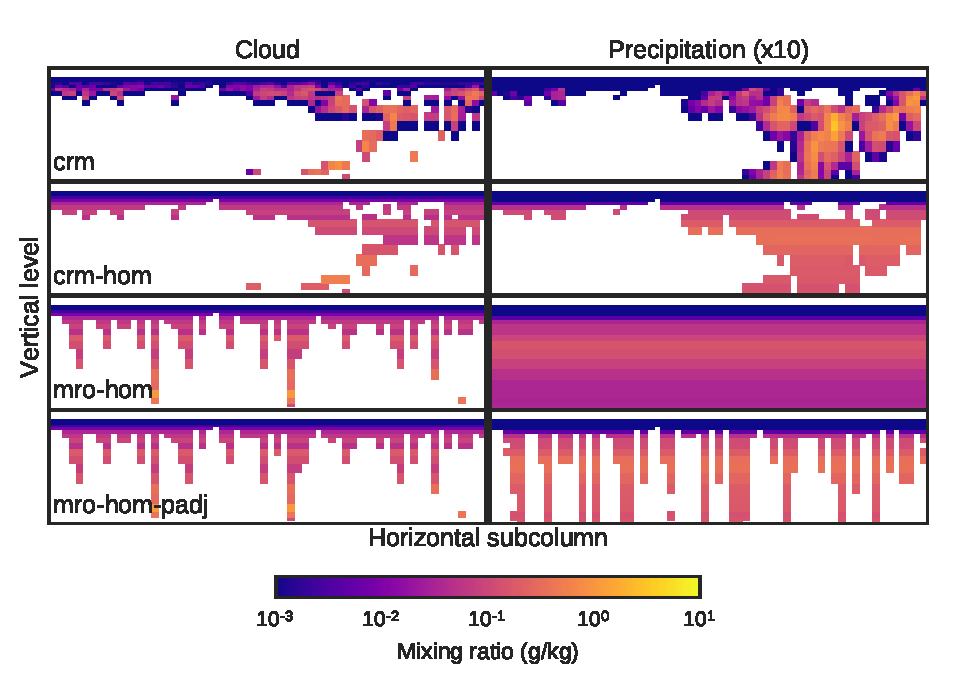
\includegraphics{graphics/subgrid1_mxratio_example.pdf}
\caption{\label{fig:subgrid1_mxratio_example}Total cloud (left) and
precipitation (right) mixing ratios from the original CRM fields (top),
homogenized CRM fields (CRM-HOM, second row), regenerated using
SCOPS/PREC\_SCOPS (MRO-HOM, third row), and regenerated using
SCOPS/PREC\_SCOPS with precipitation adjusted to conform to the
precipitation fraction from the CRM (MRO-HOM-PADJ, bottom row) for an
example gridbox (00 UTC 01 July 2000, 10 N, 180
E).}\label{fig:subgrid1ux5fmxratioux5fexample}
\end{figure}

First, a set of fields with homogenized condensate (referred to as
``CRM-HOM'') is created by replacing the condensate amount in each
cloudy CRM column in each gridbox with the gridbox in-cloud average (for
each level). This is repeated for precipitation, and is done separately
for each hydrometeor type (cloud liquid, cloud ice, precipitating
liquid, precipitating ice). No change is made to the spatial (horizontal
or vertical) location of cloud and precipitation or how cloud and
precipitation overlap with one another, so this modification retains the
exact cloud and occurrence overlap from the original CRM.

A second set of modified fields (referred to as ``MRO-HOM'') is created
by first calculating the gridbox mean cloud fraction and cloud and
precipitation condensate profiles (similarly to how a GCM would
represent the clouds) and then regenerating cloud and precipitation
subcolumns using SCOPS and PREC\_SCOPS with maximum-random cloud overlap
and homogeneous condensate, as described above. Because the embedded CRM
in SP-CAM (SAM) does not distinguish between stratiform and convective
cloud and precipitation, all cloud and precipitation is passed to SCOPS
and PREC\_SCOPS as if it were stratiform.

The simulators for the passive remote sensing instruments ISCCP, MODIS,
and MISR take as input only the cloud properties, but CloudSat radar
reflectivity is extremely sensitive to the presence of precipitation
(because radar reflectivity depends on the sixth moment of the particle
size distribution), and thus the treatment of precipitation is critical
to the accurate simulation of radar reflectivity. As mentioned above,
the lack of a constraint in the PREC\_SCOPS algorithm on the fraction of
columns that are determined to be precipitating can lead to a gross
over-estimation of precipitation occurrence. This is evident from
Figure~\ref{fig:subgrid1_mxratio_example} for the example gridbox shown,
and it will be shown below that this leads to especially large errors in
simulated CloudSat radar reflectivity and diagnostics calculated from
it.

Many GCMs may not yet include precipitation fraction as model fields,
but it is available in the NCAR CAM model, and is easily calculated from
the CRM fields in the SP-CAM model output used in this study. This
enables the simple modification to the regenerated subcolumn
precipitation condensate to force the fraction of precipitating
subcolumns at any level within a gridbox to match the fraction of
precipitating CRM columns at that level in the baseline CRM fields, as
described above. An additional set of modified fields is created from
the original CRM fields (referred to as ``MRO-HOM-PADJ'') using SCOPS
with MRO, homogeneous cloud and precipitation condensate, and this
precipitation adjustment. It will be shown below that this adjustment
substantially reduces the errors in simulated CloudSat radar
reflectivity.

With this set of cases, the sensitivities of the COSP diagnostics to
both occurrence overlap and condensate heterogeniety can be separately
quantified by calculating appropriate differences between the three
cases. Because the CRM-HOM case shares the exact occurrence overlap with
the original CRM fields but uses homogenized condensate, differences in
the COSP diagnostics between the CRM-HOM case and those from the
unmodified CRM case will show the sensitivity of the COSP diagnostics to
the assumption of homogeneous cloud and precipitation condensate.
Because the MRO-HOM fields share the same homogeneous condensate
profiles as the CRM-HOM fields but with maximum-random occurrence
overlap, differences between MRO-HOM and CRM-HOM will show the
additional impact of maximum-random occurrence overlap. Lastly, the
differences between MRO-HOM and CRM will show the total error due to
using both homogeneous cloud and precipitation condensate and
maximum-random overlap (i.e., the GCM-equivalent errors expected using
both MRO and homogeneous condensate). Symbolically, for a COSP-simulated
psuedo-retrieved quantity \(X\) (i.e., MISR cloud top height), the total
error in using the subcolumn generator \(E_\textrm{total}\), the
component of the error due to using homogeneous condensate
\(E_\textrm{homogeneous}\), and the component of the error due to the
overlap assumption \(E_\textrm{overlap}\) are calculated as
\[\begin{gathered} E_\textrm{total} = X_\textrm{MRO-HOM} -
X_\textrm{CRM} \\ E_\textrm{homogeneous} = X_\textrm{CRM-HOM} - X_\textrm{CRM}
\\ E_\textrm{overlap} = X_\textrm{MRO-HOM} - X_\textrm{CRM-HOM}\end{gathered}\]
For the CloudSat-simulated radar reflectivity, the error due to the
overestimation of precipitation using the PREC\_SCOPS routine without
the precipitation adjustment can be calculated as \[\begin{gathered}
E_\textrm{precip} = X_\textrm{MRO-HOM} - X_\textrm{MRO-HOM-PADJ}\end{gathered}\]

In order to more easily evaluate the properties of the modified fields,
and to ensure a consistent treatment for each case, the modified cases
are created outside of the COSP software infrastructure, and then fed
into COSP via a standalone driver program. COSP is intended to be
implemented directly into the source code of a model, but a minimal
working driver program capable of reading in archived large-scale model
output in netCDF format and saving COSP outputs in CMOR-compliant netCDF
files is distributed with the COSP source code. In order to run COSP on
the SP-CAM output used in this study, this minimal example program was
substantially rewritten and modularized, resulting in a stand-alone
Fortran 90 program that can read standard history files from SP-CAM and
write COSP outputs in CMOR-compliant format as well.

\section{Sensitivity of simulated passive remote sensing
diagnostics}\label{sensitivity-of-simulated-passive-remote-sensing-diagnostics}

The MISR, ISCCP, and MODIS simulators estimate the cloud top heights (or
cloud top pressures, in the case of ISCCP and MODIS) that would be
retrieved by each instrument from the model input. These cloud top
heights are aggregated together with the column cloud optical depth into
joint histograms consistent with those produced by the individual
instrument teams. These diagnostic summaries provide a description of
cloud occurrence tied to their radiative impact, because the height of
cloud top affects top of atmosphere outgoing longwave emission (and
heating of the surface and atmosphere below the cloud top) and the
optical depth or brightness of clouds affects the reflectance of
shortwave energy to space (and cooling of the surface and atmosphere
below cloud top). Cloud area for specific cloud types can be calculated
from these joint histograms by summing appropriate bins in the joint
histograms.

\begin{figure}[htbp]
\centering
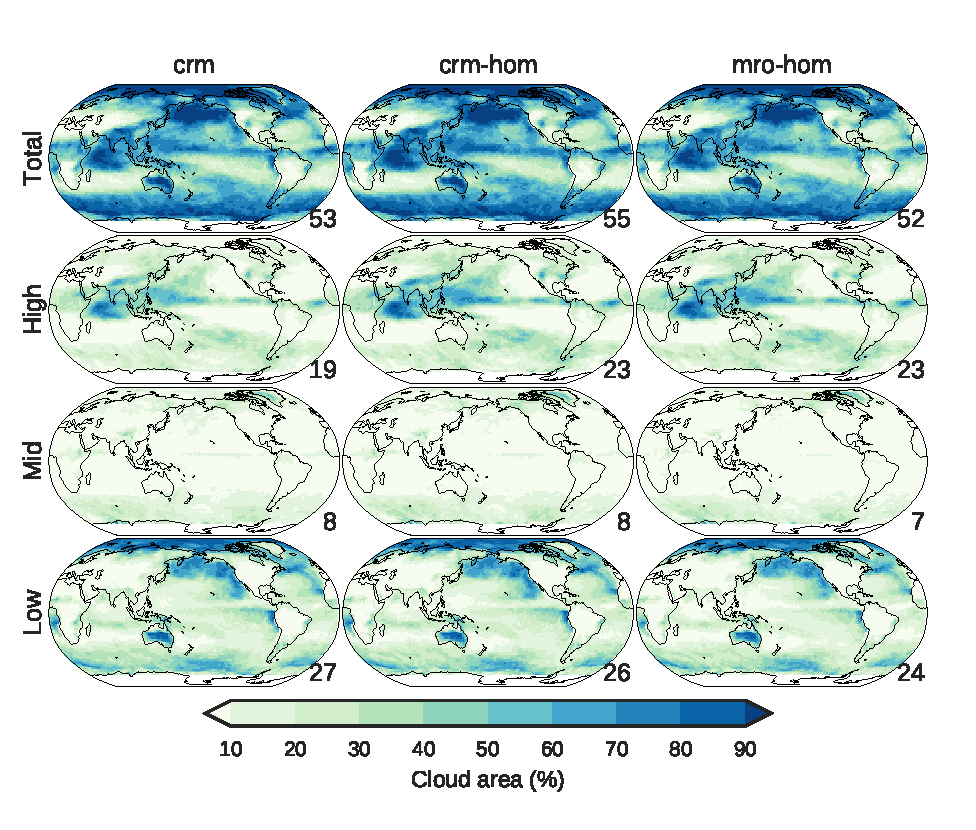
\includegraphics{graphics/subgrid1_cldmisr_maps.pdf}
\caption{\label{fig:subgrid1_cldmisr_maps}From top to bottom,
MISR-simulated total, high-topped, mid-topped, and low-topped cloud area
using the (from left to right) CRM, CRM-HOM, and MRO-HOM fields as input
to COSP.}\label{fig:subgrid1ux5fcldmisrux5fmaps}
\end{figure}

Figure~\ref{fig:subgrid1_cldmisr_maps} shows MISR-simulated monthly-mean
total (optical depth \(\tau > 0.3\)), high-topped (cloud top height
\(z_c > 7\) km, \(\tau > 0.3\)), mid-topped (\(3 < z_c < 7\) km,
\(\tau > 0.3\)), and low-topped (\(z_c < 3\) km, \(\tau > 0.3\)) cloud
area simulated from the baseline CRM, CRM-HOM, and MRO-HOM cases. The
spatial patterns and global means are similar between each of these
cases, and global mean values agree to within 4\% cloud area for all
cloud types. While the differences in the global means appear small, it
should be noted that this is on the order of the uncertainty in
comparisons between MISR retrievals and MISR-simulated retrievals using
CloudSat and CALIPSO-derived extinction profiles, as shown in
Section~\ref{sec:misr}. It will also be shown in Section~\ref{sec:cmip5}
that mid and high-topped clouds in many of the CMIP5 models have global
mean biases on the order of 5\% cloud area, so these errors are
comparable and thus important, despite being small relative to the total
cloud area.

\begin{figure}[htbp]
\centering
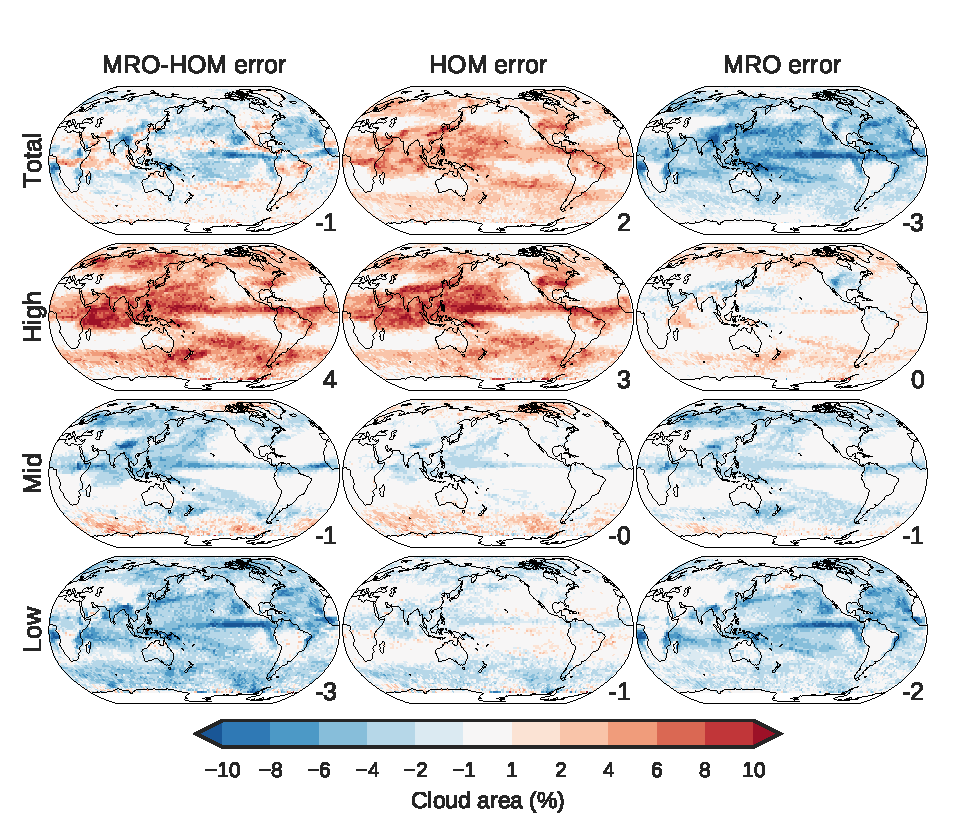
\includegraphics{graphics/subgrid1_cldmisr_maps_diff.pdf}
\caption{\label{fig:subgrid1_cldmisr_maps_diff}Errors in MISR-simulated
cloud area by cloud type for (from top to bottom) total, high-topped,
mid-topped, and low-topped clouds. Shown are (from left to right) the
total error in using SCOPS/PREC\_SCOPS with homogeneous cloud
condensate, the component of the error due only to homogenizing the
condensate, and the component of the error due only to using SCOPS to
regenerate subcolumns with maximum-random
overlap.}\label{fig:subgrid1ux5fcldmisrux5fmapsux5fdiff}
\end{figure}

Large regional errors emerge when differences are calculated, and when
those differences are broken into components due to homogenizing the
clouds and to the treatment of cloud occurrence overlap following the
framework described in Section~\ref{sec:subgrid1Framework}.
Figure~\ref{fig:subgrid1_cldmisr_maps_diff} shows the total error in
regenerating condensate from gridbox-means using SCOPS/PREC\_SCOPS
(outputs from MRO-HOM minus outputs from CRM, left column), as well as
the components of these errors due separately to homogenizing the cloud
condensate within each gridbox (HOM errors; CRM-HOM minus CRM, middle
column), and using the maximum-random overlap assumption to re-generate
subcolumns from the grid-box means (MRO errors; MRO-HOM minus CRM-HOM,
right column). Errors in MISR-simulated total cloud area due to
homogenizing the cloud and precipitation condensate (top row, middle
panel) are everywhere positive. By homogenizing the cloud condensate,
the total number of CRM columns that contain cloud condensate have not
actually been changed, nor have those columns been re-arranged in any
way. Rather, the increase in the simulated total cloud area is explained
in terms of how ``cloud'' is defined using the MISR simulator outputs.
In order to make more reasonable comparisons with satellite
observations, which have finite detection capabilities, columns are
considered cloudy only if the total column optical depth exceeds some
threshold value, nominally \(\tau > 0.3\). Homogenizing the condensate
changes the distribution of optical depth. This happens because CRM
columns with low condensate amounts (and thus lower resulting optical
depths) often occur alongside columns with larger condensate amounts
within the same gridbox, such that taking the average results in a
squeezing of the distribution of condensate (less occurrence in the
tails of the distribution and more near the mode), so a greater number
of columns exceed the optical depth threshold. This effect is
illustrated in Figure~\ref{fig:subgrid1_cldtau_distribution}, which
shows the distribution (histogram) of cloud optical depth for a single
time-step of SP-CAM output. The increase in total cloud area due to this
effect is modest, and only results in an increase of 2\% cloud area in
the global mean and regional errors on the order of 4-6\% cloud area, as
seen in Figure~\ref{fig:subgrid1_cldmisr_maps_diff}. Errors due to this
effect are larger for the diagnosis of high-topped cloud area, and can
exceed 8-10\% cloud area in the deep tropics, especially over the
Tropical Warm Pool region over the Maritime Continent and over the
Indian Ocean. These regions are dominated by deep convective cloud
systems with associated cirrus anvils consisting of high, thin ice
clouds with very low optical depths. This situation is especially
conducive to the effect illustrated in
Figure~\ref{fig:subgrid1_cldtau_distribution}, due to the increased
likelihood of averaging columns with optical depths that would be below
the threshold with those having much larger optical depths. {[}should
comment on increase of optically thick cloud due to this effect as
well{]}

\begin{figure}[htbp]
\centering
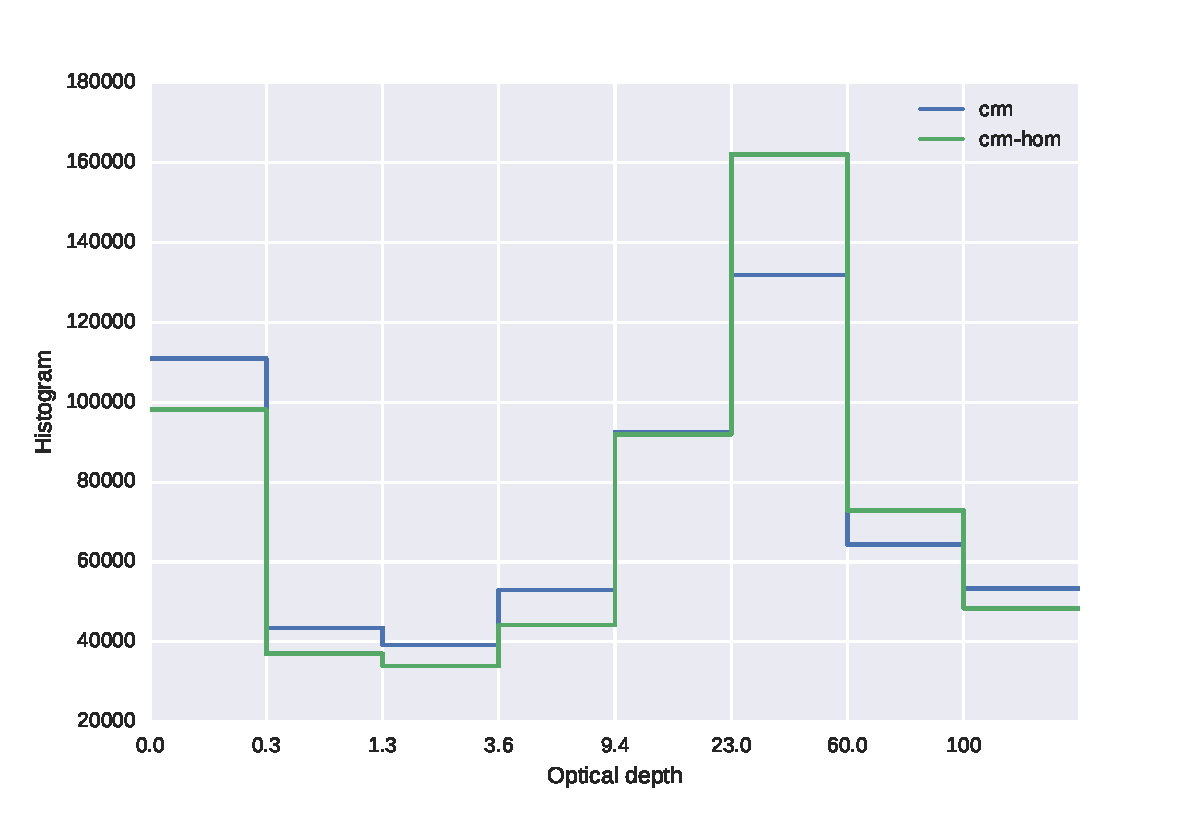
\includegraphics{graphics/taudist_hom.pdf}
\caption{\label{fig:subgrid1_cldtau_distribution}Marginal histogram of
cloud optical depth for a single day from the CRM and CRM-HOM
cases.}\label{fig:subgrid1ux5fcldtauux5fdistribution}
\end{figure}

The errors in total cloud area from the maximum-random overlap
assumption alone are everywhere negative, showing that implementing
maximum-random overlap tends to decrease the total vertically projected
cloud area. The decrease in cloud area is a result of the maximum-random
overlap assumption tending to overestimate the vertical correlation in
adjacent cloudy layers, as discussed above and shown by previous authors
\citep{mace_and_benson-troth_2002, hogan_and_illingworth_2000, barker_2008}.
This will be explored more quantitatively in Section~\ref{sec:subgrid2}.
The decrease is only -3\% cloud area in the global mean, but can reach
values exceeding -10\% regionally, especially in the tropics. The
decrease is largest for the low-topped cloud area, and high-topped cloud
area actually increases slightly throughout some regions in middle to
high latitudes. This is because the MISR simulator includes the tendency
for MISR to ``see through'' optically thin upper cloud layers and
retrieve cloud top heights of optically thicker lower cloud layers in
cases involving multiple cloud layers. This is based on an optical depth
threshold, where upper layers below a certain optical depth threshold
are considered transparent, while layers above a certain threshold are
opaque. Because increasing vertical correlation of cloudy layers tends
to increase the cloud water path (and hence the cloud optical depth of
those combined layers), the MRO assumption inflates the high-topped
cloud area while decreasing the low-topped cloud area.

The errors in MISR-simulated cloud area due separately to homogenizing
cloud condensate and using MRO are mostly compensatory, resulting in
smaller errors in the total cloud area, but combine to produce larger
errors in high, middle, and low-topped cloud area. The effect on
simulated high-topped clouds due to the two components of the error are
both positive in sign, so that these components of the error combine to
produce much larger errors in simulated high-topped cloud, with a 5\%
cloud area increase in the global mean and an increase greater than 10\%
cloud area throughout much of the deep tropics. The errors in
high-topped cloud area are mostly compensated by a decrease in
low-topped cloud, caused primarily by the errors due to using
maximum-random overlap. The result is a decrease in simulated low-topped
cloud of 4\% cloud area in the global average that, combined with the
2\% cloud area decrease in mid-topped clouds, nearly completely
compensates the increase in high-topped cloud area.

\begin{figure}[htbp]
\centering
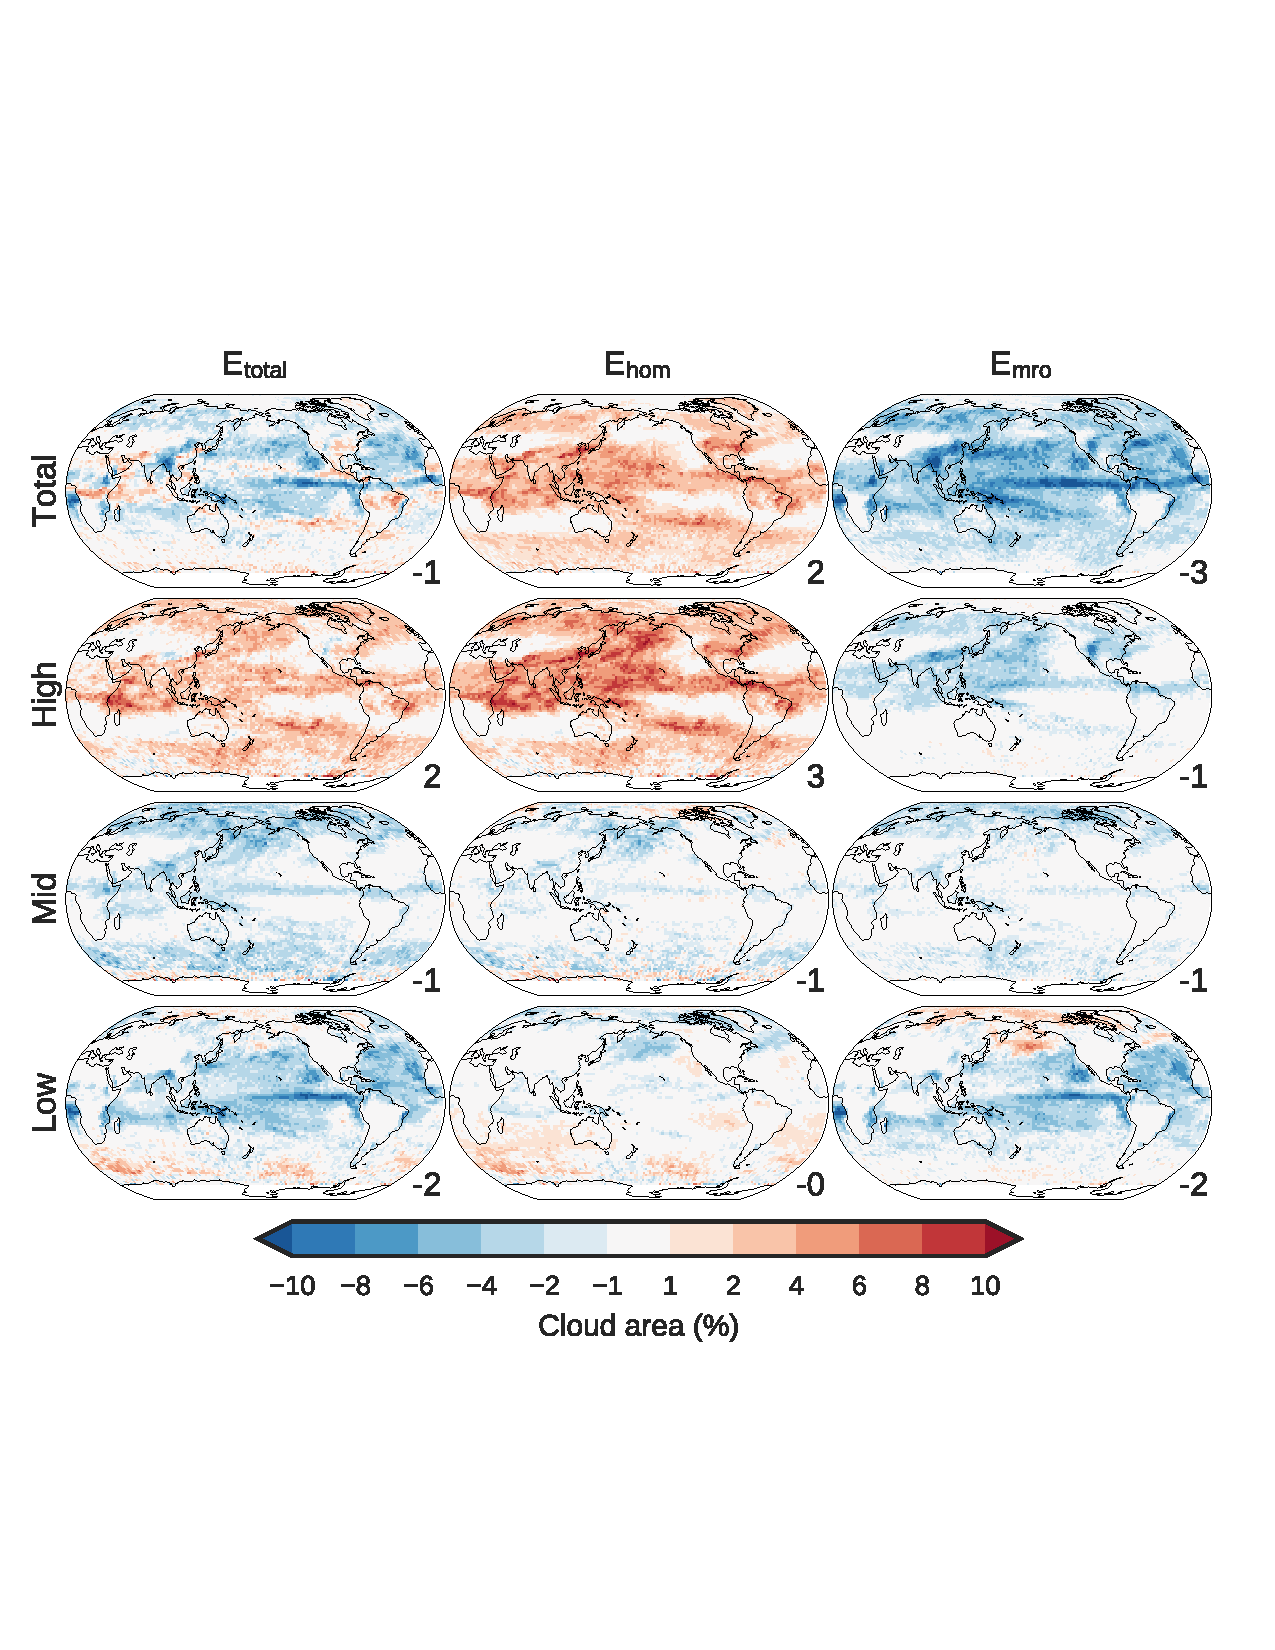
\includegraphics{graphics/subgrid1_cldisccp_maps_diff.pdf}
\caption{\label{fig:subgrid1_cldisccp_errors}Errors in ISCCP-simulated
cloud area by cloud type for (from top to bottom) total, high-topped
(\(p_c < 440\) hPa), mid-topped (\(680 < p_c < 440\) hPa), and
low-topped clouds (\(p_c > 680\) hPa). Shown are (from left to right)
the total error in using SCOPS/PREC\_SCOPS with homogeneous cloud
condensate, the component of the error due only to homogenizing the
condensate, and the component of the error due only to using SCOPS to
regenerate subcolumns with maximum-random
overlap.}\label{fig:subgrid1ux5fcldisccpux5ferrors}
\end{figure}

Figure~\ref{fig:subgrid1_cldisccp_errors} shows errors in
ISCCP-simulated cloud area by cloud type. These errors are qualitatively
similar to the errors shown in
Figure~\ref{fig:subgrid1_cldmisr_maps_diff} for the MISR simulated cloud
area by cloud type, with again an overestimation of total and
high-topped cloud area due to homogenizing cloud condensate and an
underestimation of total and low-topped cloud area due to using
maximum-random overlap. The errors in high-topped cloud area due to
homogenizing condensate is similar to the errors in the MISR-simulated
cloud area, but the errors due to using MRO are somewhat different
between the ISCCP and MISR-simulated high-topped cloud area.
MISR-simulated high-topped cloud area was actually increased somewhat in
some regions when using the MRO, but ISCCP-simulated high-topped cloud
area is universally decreased when using MRO. This results in a lower
error in ISCCP-simulated high-topped cloud due to the combined effects
of homogenizing cloud condensate and using MRO due to compensating
errors between the two effects.

\section{Sensitivity of simulated CloudSat
diagnostics}\label{sensitivity-of-simulated-cloudsat-diagnostics}

\begin{figure}[htbp]
\centering
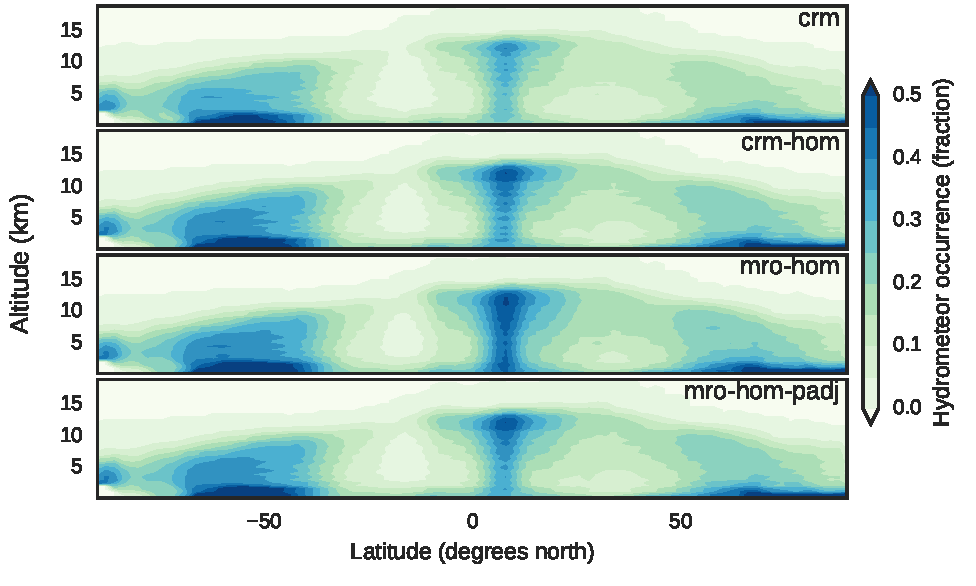
\includegraphics{graphics/subgrid1_hfba_zonal.pdf}
\caption{\label{fig:subgrid1_hfba_zonal}Zonal-mean hydrometeor occurence
fraction by height}\label{fig:subgrid1ux5fhfbaux5fzonal}
\end{figure}

\begin{figure}[htbp]
\centering
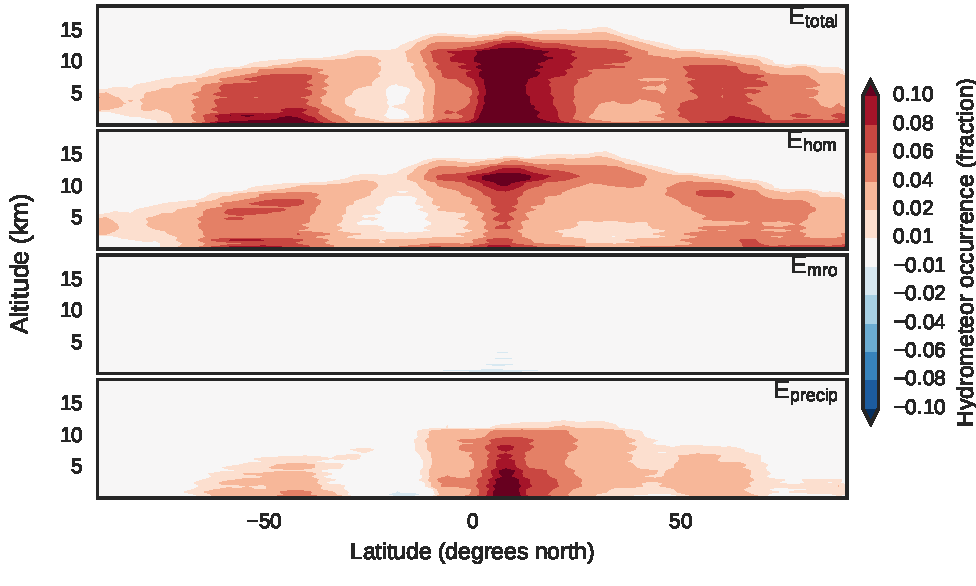
\includegraphics{graphics/subgrid1_hfba_zonal_diff.pdf}
\caption{\label{fig:subgrid1_hfba_zonal_diff}Zonal-mean hydrometeor
occurence fraction by height errors. {[}TODO: rename `MRO error' to
something less misleading\ldots{}this panel includes errors due to
precip, which are shown
below.{]}}\label{fig:subgrid1ux5fhfbaux5fzonalux5fdiff}
\end{figure}

The 94 GHz radar reflectivity (\(Z_e\)) retrieved by the CloudSat Cloud
Profiling Radar (CPR) is simulated in COSP using the Quickbeam
\citep{haynes_et_al_2007} radar simulator. Quickbeam accounts for
attenuation due to both hydrometeors and gases in the atmosphere between
the detector (radar) and the hydrometeors for which cloud properties are
being ``retrieved''. Because the CloudSat cloud radar has difficulty
detecting hydrometeors with reflectivities below -27.5 dBZ, this
threshold is often used when comparing simulated reflectivities from
models to CloudSat observations \citep{marchand_et_al_2009}. The
fraction of profiles with radar reflectivities above this threshold can
be taken as a measure of the ``hydrometeor occurrence'' (fraction of
radar volumes containing either cloud or precipitation, or both).

Figure~\ref{fig:subgrid1_hfba_zonal} shows simulated zonal-mean
hydrometeor occurrence profiles (the sum of occurrences of radar
reflectivity bins with reflectivity \(Z_e > -27.5\) dBZ at a given
height) from the CloudSat simulator using the CRM, CRM-HOM, MRO-HOM, and
MRO-HOM-PADJ fields, and Figure~\ref{fig:subgrid1_hfba_zonal_diff} shows
the errors in the MRO-HOM fields as well as the components of the errors
due separately to homogenizing the condensate amounts and in using the
maximum-random overlap assumption. Homogenizing the cloud and
precipitation condensate amounts and using the subcolumn generator in
COSP both result in an increase in simulated hydrometeor occurrence at
all altitudes. These errors are especially large in the deep tropics in
the ITCZ and in both northern and southern hemisphere mid-latitudes. The
bottom panel of Figure~\ref{fig:subgrid1_hfba_zonal_diff} shows the
component of the error due to using the unconstrained precipitation
treatment, and it is clear that this error accounts for the majority of
the error diagnosed in the panel above as due to using SCOPS/PREC\_SCOPS
to regenerate subcolumns. The errors due separately to homogenizing
cloud and precipitation and to using the MRO scheme in COSP combine to
produce larger total errors in hydrometeor occurrence than result from
either component alone (top panel of
Figure~\ref{fig:subgrid1_hfba_zonal_diff}).

These errors in hydrometeor occurrence are understand more fully by
looking at the full reflectivity with height histograms.
Figure~\ref{fig:subgrid1_cfadDbze94_tropics} shows the simulated radar
reflectivity with height histograms using the CRM, CRM-HOM, MRO-HOM, and
MRO-HOM-PADJ cases for the northern hemisphere tropics (0 to 5 N
latitude). This region is chosen because of the large errors evident in
Figure~\ref{fig:subgrid1_hfba_zonal_diff}. While the histograms all show
similar patterns of high frequency along a characteristic curve typical
of reflectivity with height histograms
\citep[e.g.;][]{marchand_et_al_2009}, the homogenized cases show
enhanced occurrence along the characteristic curve, and suppressed
occurrence off of it where baseline occurrences are lower. This is
clearer in Figure~\ref{fig:subgrid1_cfadDbze94_tropics_diff}, which
shows errors due to using homogeneous clouds and precipitation and to
using SCOPS/PREC\_SCOPS to regenerate subcolumns. Similar to the errors
in MISR-simulated cloud area, the source of these errors is driven by
the squeezing of the distribution of condensate that results from
replacing the subgrid distributions of condensate with the gridbox
averages, which effectively reduces the tails of the distribution by
removing the within-gridbox variability. This explains the apparent
increase from low reflectivities to high reflectivities, but it would be
expected that this would be accompanied by a corresponding decrease in
the occurrence of very large reflectivities, which is \emph{not} seen in
Figure~\ref{fig:subgrid1_cfadDbze94_tropics_diff}.

\begin{figure}[htbp]
\centering
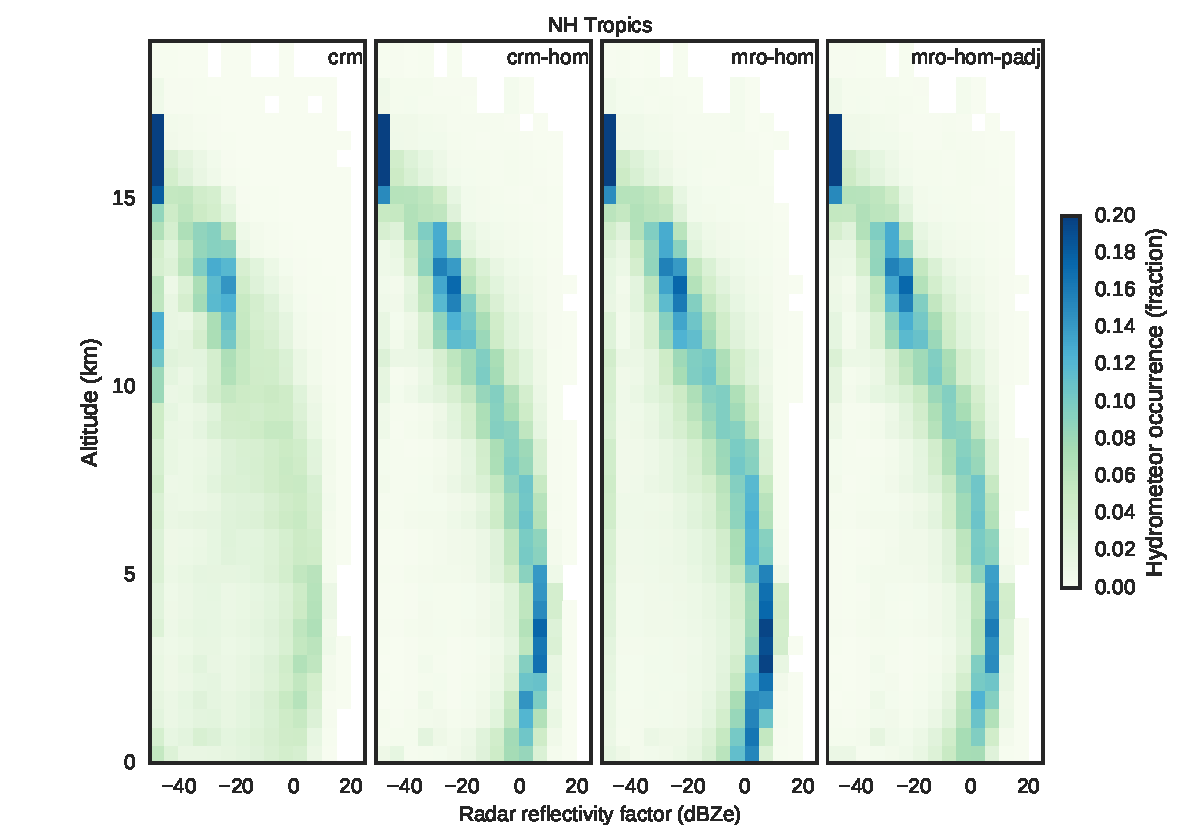
\includegraphics{graphics/subgrid1_cfadDbze94_NHTropics.pdf}
\caption{\label{fig:subgrid1_cfadDbze94_tropics}Reflectivity with height
histograms for the NH Tropics
{[}\ldots{}{]}.}\label{fig:subgrid1ux5fcfadDbze94ux5ftropics}
\end{figure}

\begin{figure}[htbp]
\centering
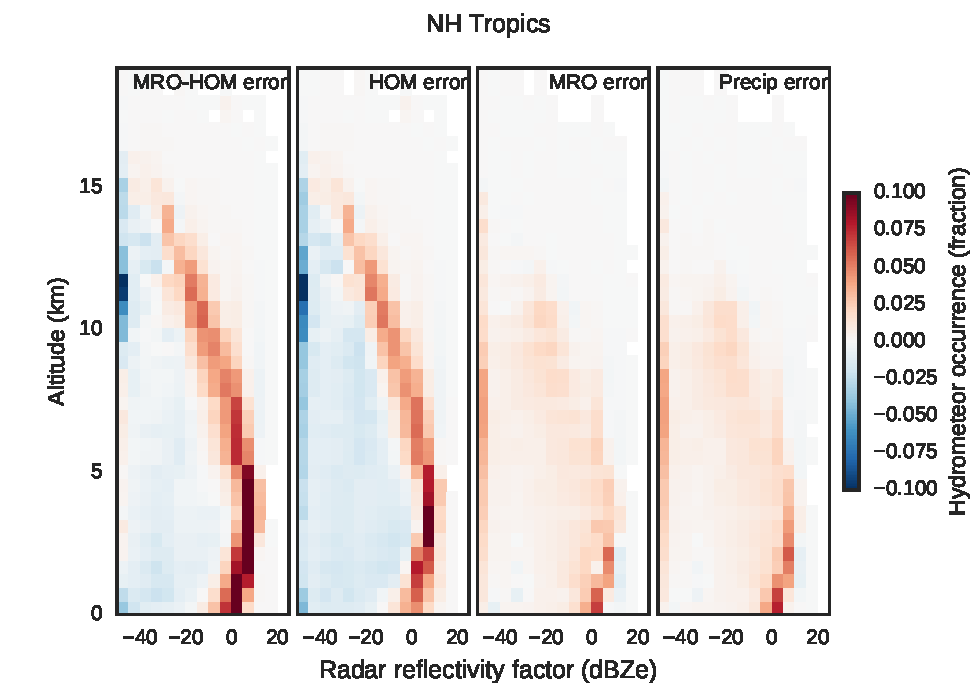
\includegraphics{graphics/subgrid1_cfadDbze94_NHTropics_diff.pdf}
\caption{\label{fig:subgrid1_cfadDbze94_tropics_diff}Errors in
reflectivity with height histograms for the NH Tropics
{[}\ldots{}{]}.}\label{fig:subgrid1ux5fcfadDbze94ux5ftropicsux5fdiff}
\end{figure}

This apparent inconsistency is explained by considering the attenuation
of the radar signal by hydrometeors existing between each radar volume
and the detector. The presence of such hydrometeors tends to decrease
the radar signal, and in the presence of hydrometeors with large
reflectivities this effect can be quite large. Because homogenizing the
cloud and precipitation condensate decreases precisely those
hydrometeors that would be expected to have such large reflectivities,
homogenizing tends to simultaneously decrease the attenuation. Thus,
while the total number of these highly reflective hydrometeors is
decreased in the homogenized case, more of them would actually be
visible to the radar due to decreased attenuation. The result is that
the occurrence is increased along the characteristic curve, decreased
for hydrometeors with lower reflectivity, but essentially unchanged for
hydrometeors with large reflecitivity. This is demostrated for an
example gridbox in Figure~\ref{fig:subgrid1_cfadDbze94_testatt}, which
shows the simulated reflectivity from both the CRM and CRM-HOM fields,
but with attenuation turned on (top), and with attenuation turned off
(bottom) for comparison. The histograms with attenuation turned off show
precisely the squeezing of the distribution that we would have expected
in the absence of attenuation.

\begin{figure}[htbp]
\centering
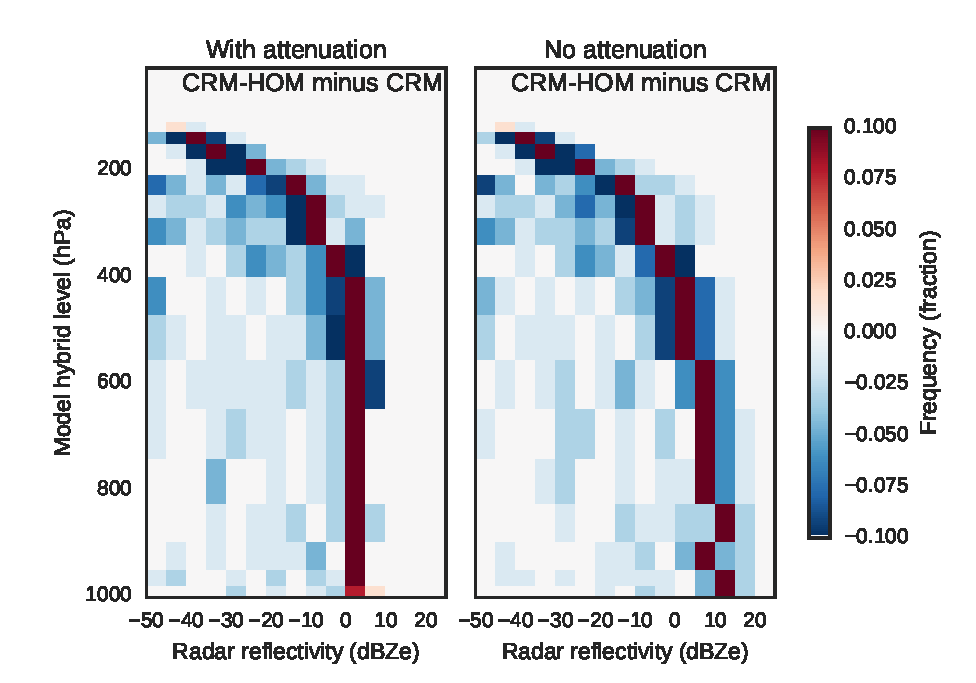
\includegraphics{graphics/subgrid1_cfadDbze94_att-test.pdf}
\caption{\label{fig:subgrid1_cfadDbze94_testatt}Differences in simulated
reflectivity with height histograms between CRM and CRM-HOM cases for an
example gridbox (the same gridbox shown in
Figure~\ref{fig:subgrid1_mxratio_example}), with attenuation turned on
(left) and with attenuation turned off
(right).}\label{fig:subgrid1ux5fcfadDbze94ux5ftestatt}
\end{figure}

Errors in CloudSat-simulated hydrometeor occurrence due to using the
SCOPS/PREC\_SCOPS subcolumn scheme to re-generate the subcolumns are
less extensive than the errors due to homogenizing the hydrometeor
properties, but can exceed 10\% frequency of occurrence in the tropics,
and again lead to a false increase in the total hydrometeor occurrence.
Figure~\ref{fig:subgrid1_cfadDbze94_tropics_diff} shows that the error
is due to an increase in the occurrence of hydrometeors with all
reflectivities, but especially due again to an increase in the
occurrence of columns with simulated radar reflectivity factor along the
characteristic curve. The effect is more pronounced at low to mid-levels
(altitude \(z < 5\) km). This error is not surprising given the
discussion in Section~\ref{sec:subgrid1Framework} in the context of
Figure~\ref{fig:subgrid1_mxratio_example}, which shows that the
PREC\_SCOPS subcolumn precipitation generator can tend to overestimate
the number of precipitating subcolumns. The fourth panel of
Figure~\ref{fig:subgrid1_cfadDbze94_tropics_diff} shows the component of
the error due to using the unconstrained precipitation treatment in
PREC\_SCOPS (the difference between MRO-HOM and MRO-HOM-PADJ). This
shows that the overestimation of precipitation fraction that arises by
using PREC\_SCOPS without constraining the number of precipitating
columns to match the precipitation fraction is responsible for the
majority of the error, and the MRO error can be greatly reduced by
constraining the number of precipitating subcolumns to match a
prescribed precipitation fraction. Likewise, the errors in simulated
reflectivity with height due to the MRO alone are also small when the
precipitation is constrained by the input precipitation fraction (not
shown), leaving the homogeneous errors as dominating the total error in
simulated CloudSat radar reflectivity. This suggests that the simulated
CloudSat radar reflectivity is not sensitive to the cloud overlap, but
is sensitive to the treatment of subgrid-scale precipitation.

\section{Summary and discussion}\label{sec:subgrid1Summary}

Current global models do not resolve individual cloud elements, but
rather represent the large-scale statistics by way of parameterization.
But simulated satellite diagnostics (and radiative fluxes and heating
rates) depend on the small-scale details of clouds. This chapter has
presented an evaluation of the sensitivity of simulated MISR and
CloudSat satellite diagnostics from the CFMIP Observation Simulator
Package to two assumptions: that cloud and precipitation properties are
horizontally uniform on the scale of GCM gridboxes, and that individual
cloud elements follow a maximum-random overlap. Because these
assumptions are used to infer subgrid-scale cloud structure in model
radiative transfer codes, these assumptions are used by default in COSP
to generate stochastic subcolumns on which the individual satellite
instrument simulators are performed. However, others have shown that
these assumptions lead to biases in calculated fluxes and heating rates,
and it has been shown here that these assumptions also affect simulated
MISR and CloudSat satellite diagnostics.

The assumption of homogeneous cloud properties tends to inflate the
simulated MISR cloud area (when counting all clouds with an optical
depth greater than 0.3) because columns with small optical depths in the
tail of the distribution are sometimes shifted to values above the
cut-off threshold by averaging with columns with larger optical depths.
These errors occur primarily in high-topped clouds, and high-topped
cloud occurrence can be overestimated by as much as 10\% cloud area in
regions with a lot of high-topped optically thin cloud, such as in the
tropical western pacific and other parts of the deep tropics. The global
mean high-topped cloud error due to homogenizing the cloud properties is
about 3\% cloud area, and the effect on total cloud area is only 2\%.
The maximum-random overlap assumption tends to decrease the cloud cover
because it overestimates the vertical alignment of vertically continuous
clouds
\citep{mace_and_benson-troth_2002, hogan_and_illingworth_2000, barker_2008}.
This leads to a global mean underestimate in total cloud area of only
3\%, but with regional errors as large as 10\% cloud area, especially in
the deep tropics. The errors in cloud area due to homogeneous cloud
properties and using the maximum-random overlap are generally opposite
in sign, and result in a partial cancellation on the total error. The
result is that the errors in total cloud area are less than 2\% in the
global average, and regional errors in total cloud area are much smaller
than for either of the two components of the error. However, errors in
high and low-topped cloud area due to the two components are additive,
such that the total errors in high and low-topped clouds are larger than
they are for either the homogeneous or MRO components. High-topped cloud
is overestimated by 5\% cloud area, and low-topped cloud is
underestimated by 4\% cloud area in the global mean. Regional errors are
even larger, and high-topped cloud errors reach 10\% cloud area or more,
especially in the tropical western pacific, the Indian Ocean, and
throughout the tropics.

The sensitivity in MISR-simulated total cloud area identified here is
generally less than errors in cloud area identified in current GCMs
\citep{kay_et_al_2012, klein_et_al_2013, bodas-salcedo_et_al_2011}, and
on the order of the spread in estimates of total cloud area from
satellite remote sensing retrievals \citeauthor{marchand_et_al_2010}
\citetext{\citeyear{marchand_et_al_2010}; \citealp{pincus_et_al_2012}}.
However, the regional errors in MISR-simulated cloud area by cloud top
height identified here are large, and exceed the uncertainty in
MISR-retrieved high-topped cloud area, which is estimated to be on the
order of 5\% cloud area regionally, as shown in Section~\ref{sec:misr}.
Thus, the sensitivity of MISR-simulated cloud area to homogeneous cloud
condensate and maximum-random overlap cannot be ignored, especially as
representations of clouds in GCMs improve.

Simulated CloudSat radar reflectivity is found to be sensitive to the
treatment of unresolved subcolumn cloud and precipitation condensate
horizontal variability, but much less sensitive to the treatment of
cloud overlap. Homogenizing the cloud and precipitation condensate leads
to a narrowing of the distribution of simulated radar reflectivity,
making the more frequently occurring reflectivities in the baseline
simulation even more frequently occurring in the homogenized simulation.
This tends to decrease the occurrence of columns with small radar
reflectivity, while increasing the occurrence of columns with large
radar reflectivity. Similar to the MISR simulator, employing a
reflectivity cut-off to determine hydrometeor occurrence (for the
purpose of making consistent comparisons with CloudSat) then results in
an apparent increase in the hydrometeor occurrence when homogenizing the
cloud and precipitation properties, and an apparent increase in
precipitation occurrence. The increase in simulated hydrometeor
occurrence fraction reaches a value of 10\% in high altitudes in the
tropics and in low altitudes in mid to high-latitudes.

Using the subcolumn generator currently implemented in COSP (as of
version 1.4) leads to further errors in simulated CloudSat radar
reflectivity and hydrometeor occurrence that combine with the errors due
to homogenizing the cloud and precipitation condensate to produce even
larger total errors that reach 10\% frequency of occurrence at all
altitudes throughout the tropics. Much of this error is due to the fact
that precipitation has a relatively large reflectivity compared with
clouds, and the subcolumn precipitation scheme implemented in COSP tends
to overestimate the number of precipitating subcolumns. Using this
subcolumn scheme then tends to increase the number of columns with large
radar reflectivity, and thus increases the simulated hydrometeor
occurrence. Constraining the number of precipitating subcolumns by the
precipitation fraction greatly reduces errors in simulated hydrometeor
occurrence. The ability to constrain the subcolumn precipitation by the
precipitation fraction will be included in future versions of COSP (Y.
Zhang, personal communication). The remaining errors due to
maximum-random cloud overlap alone are small, with hydrometeor
occurrence errors everywhere less than 4\% in the zonal mean.

The errors in simulated CloudSat radar reflectivity factor and
hydrometeor occurrence due to the homogenous cloud and precipitation
assumptions are troubling, and show that subgrid-scale cloud and
precipitation variability needs to be better represented in COSP in
order to create more consistent comparisons between model-diagnosed and
satellite-retrieved cloud statistics. The following chapter explores the
possibility of reducing these errors with an improved subcolumn
generator framework, which includes both a more realistic treatment of
overlap and heterogeneous subcolumn condensate.
